\section{Big data processing paradigms}\label{Big data processing}

There are different processing paradigms that were evolved over time. It all started with Batch, then Real-time was invented and most recently Hybrid. Bellow are all of them explained with two new approaches added.


\begin{figure}[H]
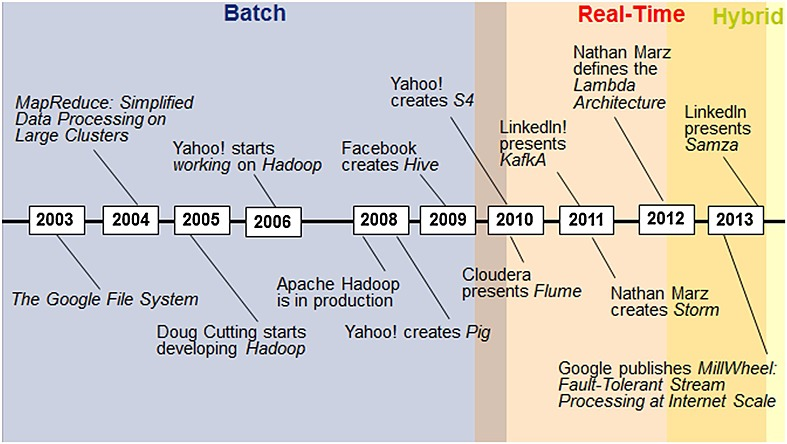
\includegraphics[scale=0.70]{img/ProcessingParadigms/Process}
\centering
\caption{Paradigms over time \parencite{casado2015emerging}}
\label{fig:Process}
\end{figure}

\subsection{Batch}\label{Batch}

Batch processing is one of the earliest processes. As name suggests, in batch processing we are expecting multiple files (batch) \parencite{web:Amazon}. Once they are received, they are being processed.

One real world example is roller coaster. In order to operate the ride in optimal capacity, we need 20 (an example number) people on it. The idea is for operator to fill the ride with 20 people. After the ride is complete, the next 20 are selected.

Similar process is in batch processing. Computer (server) waits for n number of files. After they are received, they are inserted into data pipeline in order to start the operation. Limits can be set if files are not received (but this could then be considered hybrid processing).

In our case, we are using batch processing with flamingo data. Files are downloaded from the web and once they are ready pipeline is triggered.


\begin{figure}[H]
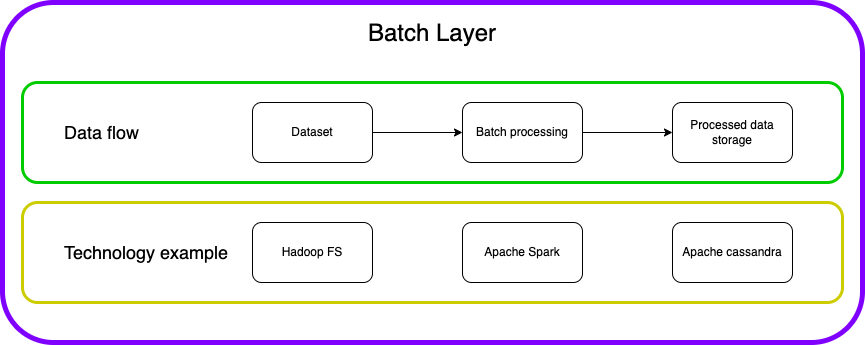
\includegraphics[scale=0.45]{img/ProcessingParadigms/BigData-Batch.png}
\centering
\caption{Batch}
\label{fig:Batch}
\end{figure}
\subsection{Real time}\label{RealTime}

Real time (or stream) processing is used when there are multiple sources feeding data all the time \parencite{wu2020reactive}.

Real world example could be water slide. There is a queue of people waiting for the ride. Operator approves each person to take a ride one after the other.  

Similarly, in stream processing, computer (server) is always waiting and ready for the files to be uploaded. We can get 1 or n number of files per second, all of them will be send to our pipeline. For example, IoT sensors. They are constantly sending the data in order to extract relevant information.

In our case, if game would be played online we would use real time operation. This is due to player movements. The rough concept would be for player to make a move, that is recorded in database and with API we would constantly getting new, updated information.


\begin{figure}[H]
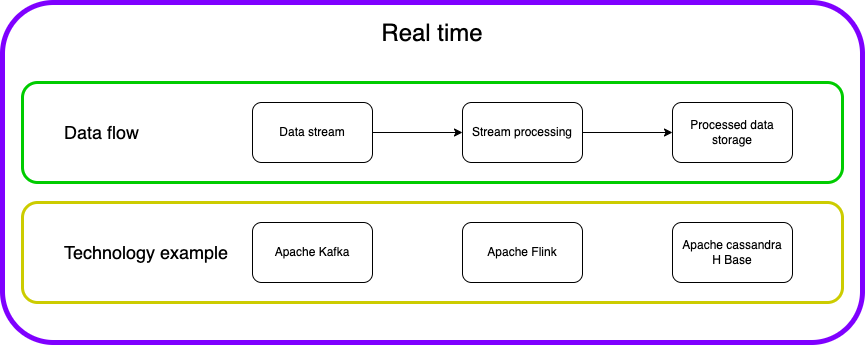
\includegraphics[scale=0.45]{img/ProcessingParadigms/BigData-RealTime.png}
\centering
\caption{Real time}
\label{fig:RealTime}
\end{figure}
\subsection{Hybrid}\label{Hybrid}

Hybrid processing is a mix of batch and real time \parencite{lewis2013content}.

Lets revisit roller coaster example. In batch scenario operator was waiting for 20 people to be seated. In hybrid scenario, we are expecting 20 people to show up. If there isn't enough people, operator will just start the ride with less than 20 people. One scenario would be business hours. In the morning and evening, we don't get as many people therefore operator is running the ride in hybrid mode but thought the noon (when there are core hours) operation seems like batch (but is hybrid on a grand scale).

Now lets consider our file ingestion from batch processing. We are still expecting n number of files. If we get n number of files, we start the processing with them (batch). Otherwise if we don't get all the files, we work with the files that were received as stream.

\begin{figure}[H]
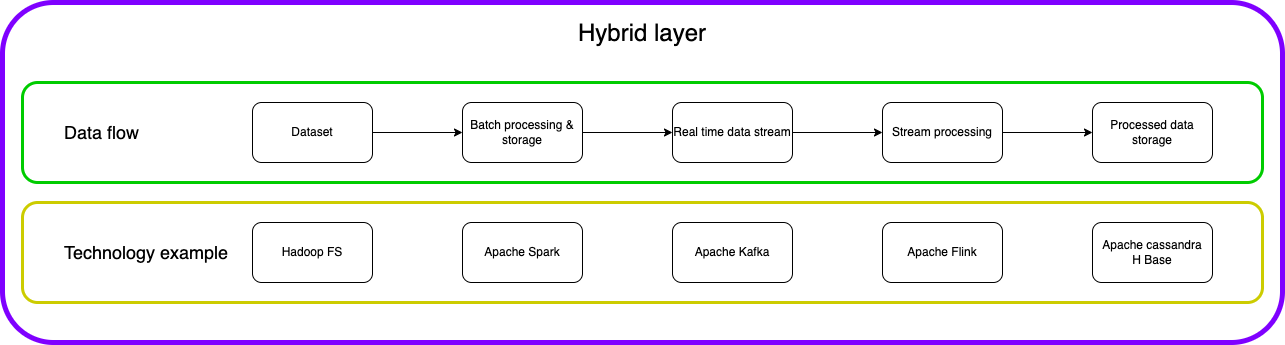
\includegraphics[scale=0.30]{img/ProcessingParadigms/BigData-HybridLayer.png}
\centering
\caption{Hybrid layer}
\label{fig:HybridLayer}
\end{figure}
\subsection{Other}\label{Other}
As technology moves on, new problems and solutions are developed. Lambda and Kappa architectures are not as popular but still interesting approaches of data pipelines.

Further discussion on Lambda and Kappa can be found under \ref{A7} and \ref{A8}.
%\subsubsection{Lambda}\label{Lambda}

Lambda is part of hybrid architecture, that means it combines batch and real time processing. Since both processes are used, it is common to split them apart. We would have batch processing for bigger files and real time (or speed) for time intense applications \parencite{lin2017lambda}.

One real world example would be airline customers. We can split them into priority and none priority. Both achieve the same goal, just one type of customers will be served first.

In our example, we could use Lambda architecture. For example, game data (how players are moving) needs to be processed in real time. But chat data can be processed as a batch. Reason for this is chat data doesn't provide as much value to us as game data.

\begin{figure}[H]
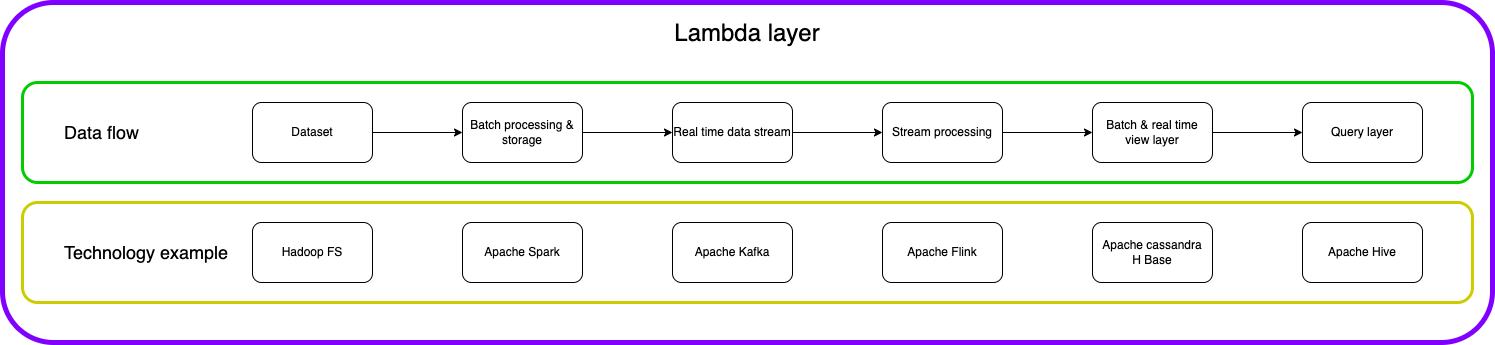
\includegraphics[scale=0.25]{img/ProcessingParadigms/BigData-Lambda.png}
\centering
\caption{Lambda}
\label{fig:Lambda}
\end{figure}

%\subsubsection{Kappa}\label{Kappa}

Kappa architecture is similar to Lambda but it has one big difference: it excludes batch processing. Arguably, it can be called another version of real time processing. If there is a batch of files send to it, they are handled as a stream of data \parencite{feick2018fundamentals}.

Since Kappa is similar to real time processing, lets reuse roller coaster example. In batch processing, we would wait for 20 people to fill the ride before operator would start the ride. In Kappa, people would still queue for the ride but as soon as the ride is available all of the people who are there would be ready to ride. In other words, our roller coaster would operate real time with the goal of less stopping regardless how many people are on the ride.

As mentioned with the real time processing, this is something that could be used with flamingo data. For example, instead of waiting for conversation between players to finish, they can directly be processed.

\begin{figure}[H]
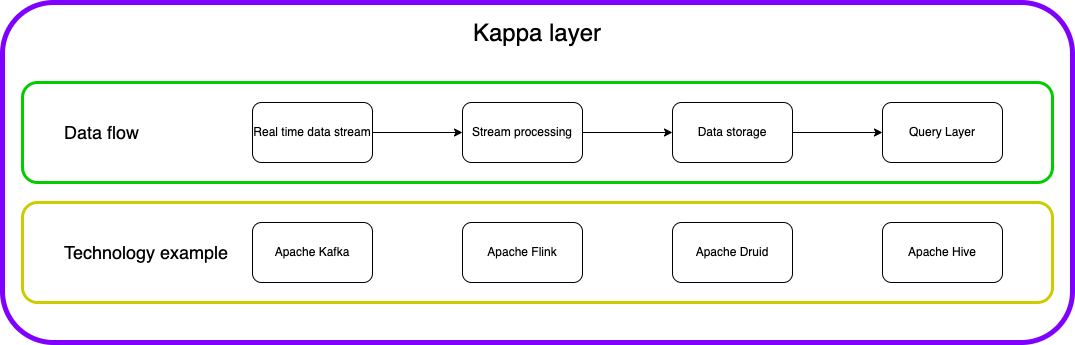
\includegraphics[scale=0.35]{img/ProcessingParadigms/BigData-Kappa.png}
\centering
\caption{Kappa}
\label{fig:Kappa}
\end{figure}


